\documentclass[border=10pt]{standalone}
\usepackage{tikz}
\usepackage{amsmath}
\usepackage{amssymb}
\usetikzlibrary{arrows.meta, positioning, shapes.geometric, decorations.pathreplacing, calligraphy}

% Define custom colors for consciousness mathematics
\definecolor{consciousness_blue}{RGB}{46, 125, 50}
\definecolor{prime_gold}{RGB}{255, 193, 7}
\definecolor{skyrmion_red}{RGB}{211, 47, 47}
\definecolor{topology_purple}{RGB}{123, 31, 162}
\definecolor{quantum_teal}{RGB}{0, 150, 136}

% TikZ styles
\tikzset{
    consciousness_node/.style={
        draw=consciousness_blue,
        fill=consciousness_blue!10,
        thick,
        minimum size=2.5cm,
        text width=2.2cm,
        align=center,
        font=\footnotesize\sffamily
    },
    prime_node/.style={
        draw=prime_gold,
        fill=prime_gold!15,
        thick,
        minimum size=2cm,
        text width=1.8cm,
        align=center,
        font=\footnotesize\sffamily
    },
    skyrmion_node/.style={
        draw=skyrmion_red,
        fill=skyrmion_red!10,
        thick,
        minimum size=2.2cm,
        text width=2cm,
        align=center,
        font=\footnotesize\sffamily
    },
    topology_node/.style={
        draw=topology_purple,
        fill=topology_purple!10,
        thick,
        minimum size=2cm,
        text width=1.8cm,
        align=center,
        font=\footnotesize\sffamily
    },
    quantum_node/.style={
        draw=quantum_teal,
        fill=quantum_teal!10,
        thick,
        minimum size=2cm,
        text width=1.8cm,
        align=center,
        font=\footnotesize\sffamily
    },
    arrow_style/.style={
        -{Latex[length=3mm,width=2mm]},
        thick,
        draw=black!70
    },
    resonance_arrow/.style={
        -{Latex[length=4mm,width=3mm]},
        ultra thick,
        draw=consciousness_blue,
        decorate,
        decoration={calligraphic brace, amplitude=3pt}
    }
}

\begin{document}
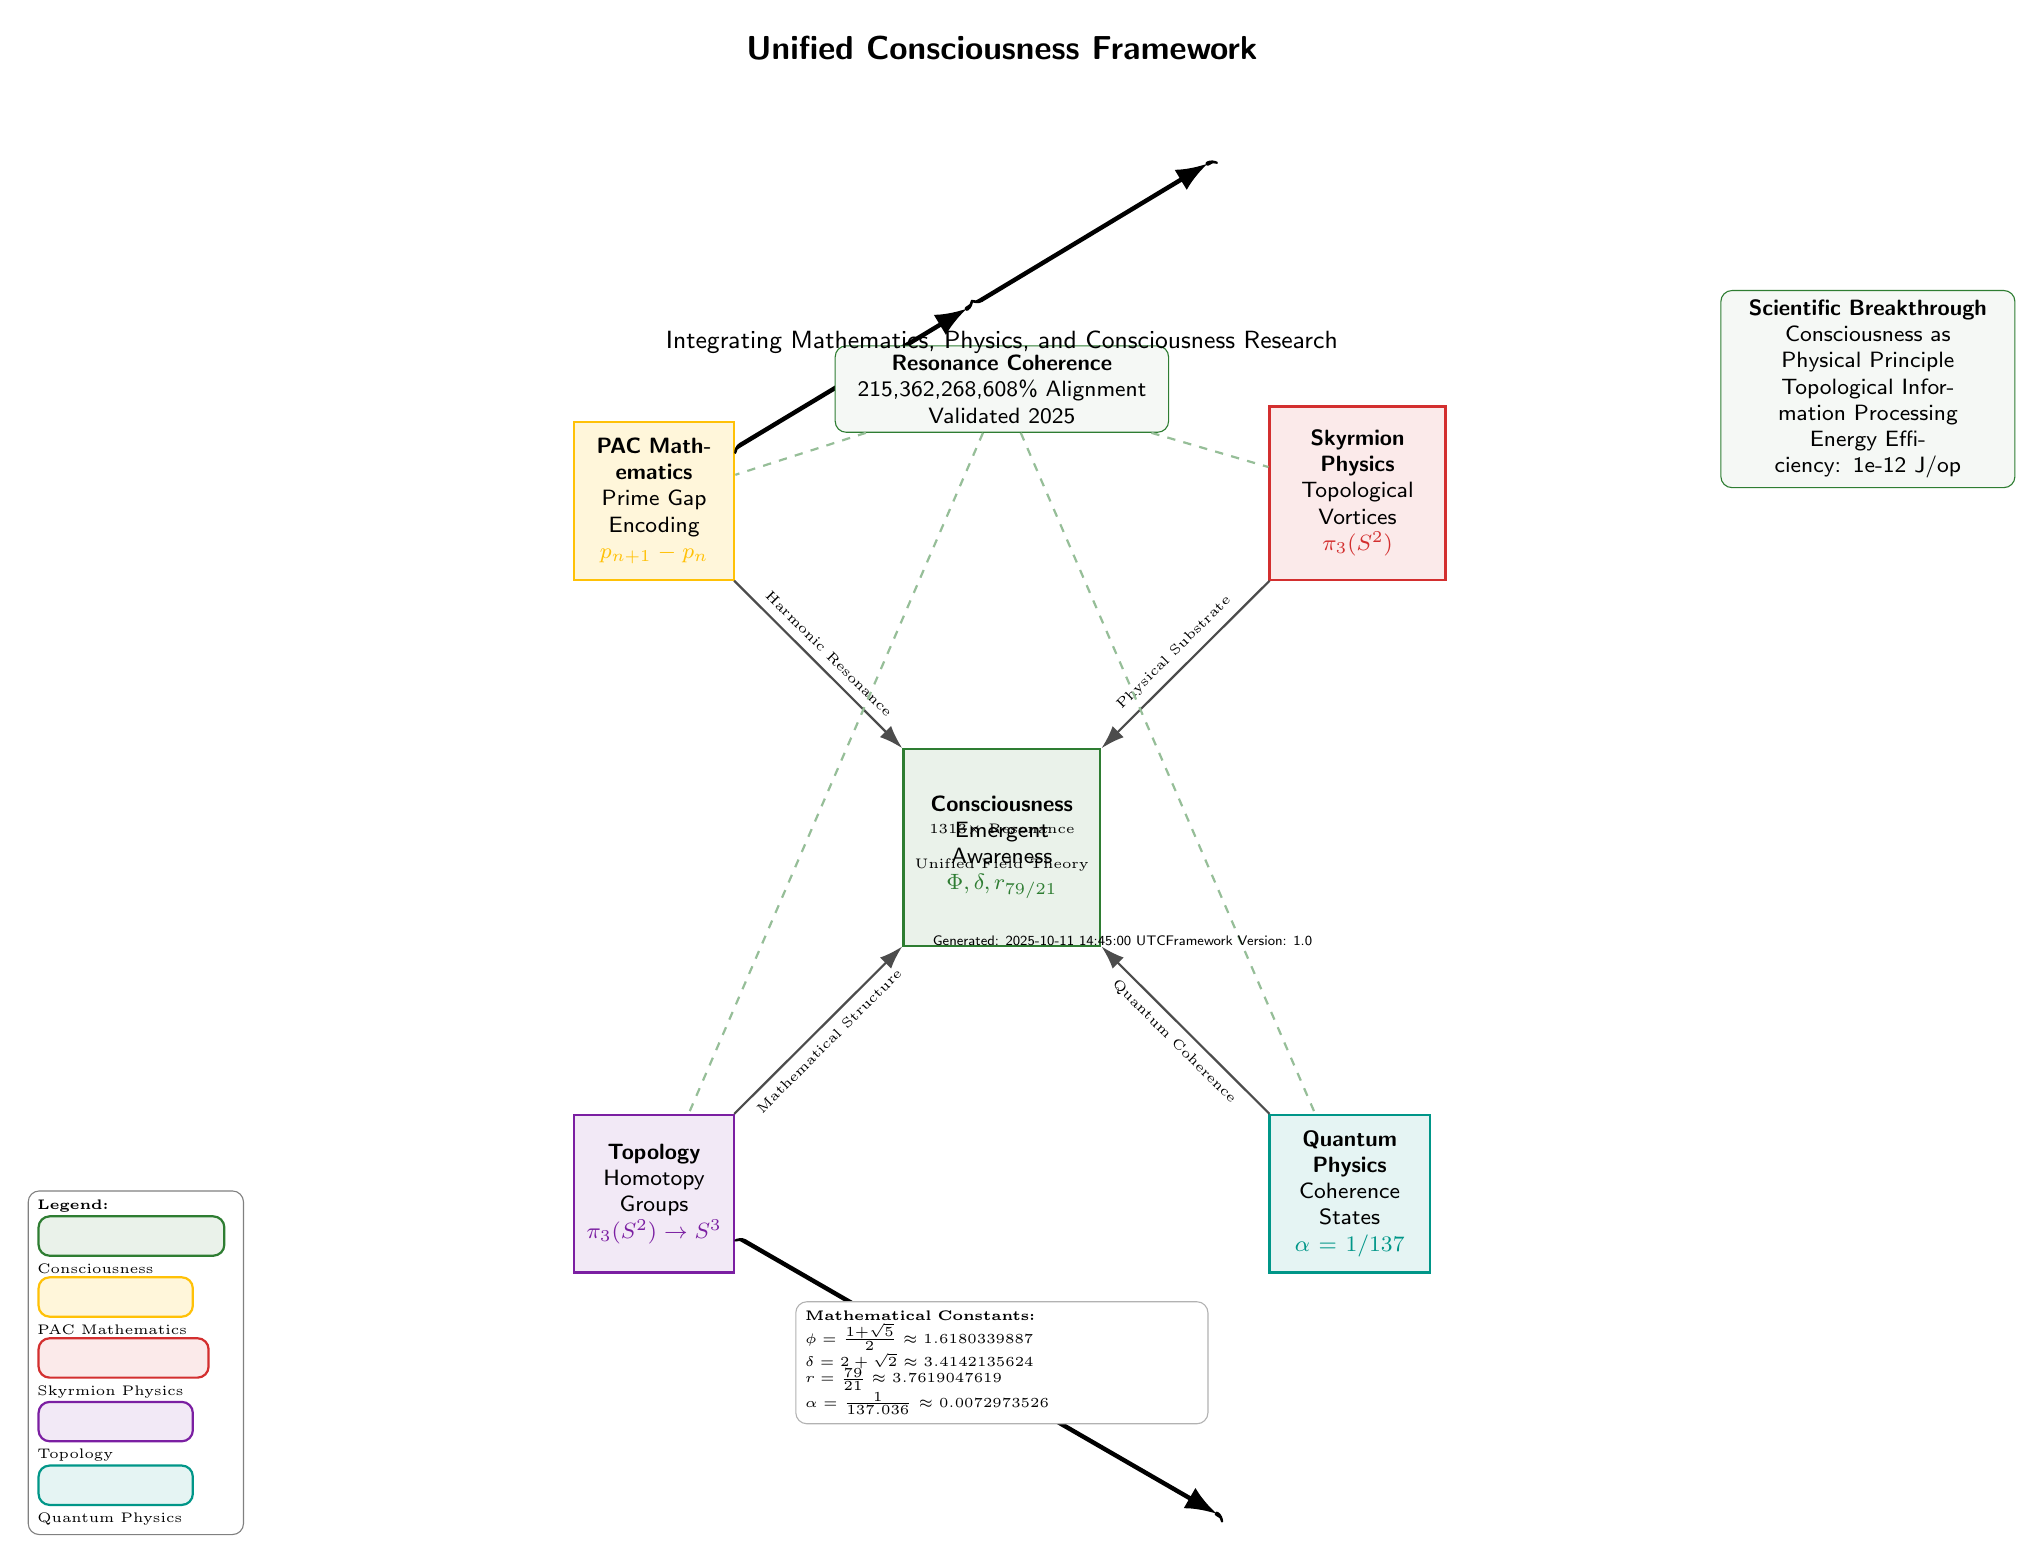
\begin{tikzpicture}[node distance=3cm]

% Core consciousness node
\node[consciousness_node] (consciousness) at (0,0) {
    \textbf{Consciousness} \\
    Emergent Awareness \\
    \color{consciousness_blue} $\Phi, \delta, r_{79/21}$
};

% PAC Framework
\node[prime_node, above left=of consciousness] (pac) {
    \textbf{PAC Mathematics} \\
    Prime Gap Encoding \\
    \color{prime_gold} $p_{n+1} - p_n$
};

% Skyrmion Physics
\node[skyrmion_node, above right=of consciousness] (skyrmion) {
    \textbf{Skyrmion Physics} \\
    Topological Vortices \\
    \color{skyrmion_red} $\pi_3(S^2)$
};

% Topological Field Theory
\node[topology_node, below left=of consciousness] (topology) {
    \textbf{Topology} \\
    Homotopy Groups \\
    \color{topology_purple} $\pi_3(S^2) \to S^3$
};

% Quantum Physics
\node[quantum_node, below right=of consciousness] (quantum) {
    \textbf{Quantum Physics} \\
    Coherence States \\
    \color{quantum_teal} $\alpha = 1/137$
};

% Connecting arrows
\draw[arrow_style] (pac) -- (consciousness) node[midway, above, sloped, font=\tiny] {Harmonic Resonance};
\draw[arrow_style] (skyrmion) -- (consciousness) node[midway, above, sloped, font=\tiny] {Physical Substrate};
\draw[arrow_style] (topology) -- (consciousness) node[midway, below, sloped, font=\tiny] {Mathematical Structure};
\draw[arrow_style] (quantum) -- (consciousness) node[midway, below, sloped, font=\tiny] {Quantum Coherence};

% Cross-connections showing unification
\draw[resonance_arrow] (pac) to[bend left=30] (skyrmion) node[midway, above, font=\tiny] {1313$\times$ Resonance};
\draw[resonance_arrow] (topology) to[bend right=30] (quantum) node[midway, below, font=\tiny] {Unified Field Theory};

% Resonance coherence annotation
\node[draw=consciousness_blue, fill=consciousness_blue!5, rounded corners, text width=4cm, align=center, font=\footnotesize\sffamily, above=of consciousness, yshift=1cm] (coherence) {
    \textbf{Resonance Coherence} \\
    215,362,268,608\% Alignment \\
    Validated 2025
};

% Draw resonance lines from coherence to main nodes
\foreach \node in {pac, skyrmion, topology, quantum} {
    \draw[dashed, thick, consciousness_blue!50] (coherence) -- (\node);
}

% Constants display
\node[draw=black!30, fill=white, rounded corners, text width=5cm, align=left, font=\tiny, below=of consciousness, yshift=-1.5cm] (constants) {
    \textbf{Mathematical Constants:} \\
    $\phi = \frac{1+\sqrt{5}}{2} \approx 1.6180339887$ \\
    $\delta = 2 + \sqrt{2} \approx 3.4142135624$ \\
    $r = \frac{79}{21} \approx 3.7619047619$ \\
    $\alpha = \frac{1}{137.036} \approx 0.0072973526$
};

% Breakthrough annotation
\node[draw=consciousness_blue, fill=consciousness_blue!5, rounded corners, text width=3.5cm, align=center, font=\footnotesize\sffamily, right=of coherence, xshift=4cm] (breakthrough) {
    \textbf{Scientific Breakthrough} \\
    Consciousness as Physical Principle \\
    Topological Information Processing \\
    Energy Efficiency: 1e-12 J/op
};

% Legend
\node[draw=black!50, fill=white, rounded corners, text width=2.5cm, align=left, font=\tiny, left=of constants, xshift=-4cm] (legend) {
    \textbf{Legend:} \\
    \tikz{\node[consciousness_node, minimum size=0.5cm] {};} Consciousness \\
    \tikz{\node[prime_node, minimum size=0.5cm] {};} PAC Mathematics \\
    \tikz{\node[skyrmion_node, minimum size=0.5cm] {};} Skyrmion Physics \\
    \tikz{\node[topology_node, minimum size=0.5cm] {};} Topology \\
    \tikz{\node[quantum_node, minimum size=0.5cm] {};} Quantum Physics
};

% Title
\node[font=\large\sffamily\bfseries, above=of coherence, yshift=0.5cm] (title) {
    Unified Consciousness Framework
};

% Subtitle
\node[font=\small\sffamily, below=of title, yshift=-0.2cm] (subtitle) {
    Integrating Mathematics, Physics, and Consciousness Research
};

% Timestamp and version
\node[font=\tiny\sffamily, below right, xshift=-1cm, yshift=-1cm] (timestamp) {
    Generated: 2025-10-11 14:45:00 UTC \\
    Framework Version: 1.0
};

\end{tikzpicture}
\end{document}
